\section{Introduction} \label{intro}

Data normalization is a fundamental preprocessing step, long recognized as essential for the stable and efficient training of neural networks. Its significance was established in early studies on neural networks optimization \citep{DBLP:series/lncs/LeCunBOM12}.
Normalization is particularly critical in time series forecasting, a domain in which deep learning models have achieved state-of-the-art performance \citep{patchtst}. Intrinsic properties of time series, such as non-stationarity, trends, and seasonality, introduce challenges that standard normalization methods fail to address \citep{adaptivenorm}.
%As a result, normalization becomes not merely a routine preprocessing step but a decisive factor influencing both model convergence and predictive performance.

Three major aspects must be considered when designing a normalization strategy for time series forecasting:

\begin{enumerate}[(i)]
    \item \textbf{Temporal distribution shift.} When training a neural forecaster over a training period, the input data distribution in a future test period may differ substantially. For instance, electricity consumption or road traffic often increase over time (see \cref{fig:shifts}).

    \item \textbf{Spatial distribution shift.} Neural forecasters are typically trained on multiple time series and must generalize to unseen time series at inference. Even when series describe similar phenomena (e.g., solar power generation at different locations), their overall distributions may differ, for example, due to scale or level shifts (see \cref{fig:shifts}).

    % \item \textbf{Conditional distribution shift.} A neural forecaster maps a look-back window to a horizon window, $f_{\theta}: \boldsymbol{x}^{\text{look-back}} \to \boldsymbol{x}^{\text{horizon}}$. The conditional distribution $p(\boldsymbol{x}^{\text{horizon}} | \boldsymbol{x}^{\text{look-back}})$ may vary both in space and time. This shift remains particularly challenging to handle (see \cref{fig:c}).
    \item \textbf{Conditional distribution shift.} A neural forecaster maps past \textit{look-back} windows to future \textit{horizon} windows. The conditional distribution of the horizon given the look-back may vary both in space and time. This shift remains particularly challenging to handle (see \cref{fig:shifts}).
\end{enumerate}



\begin{figure}[t]
    \centering
    \begin{minipage}[t]{0.31\textwidth}
        \centering
        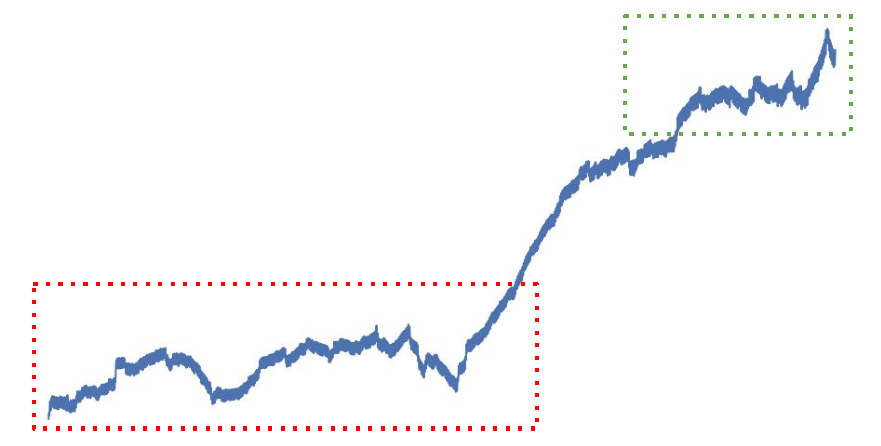
\includegraphics[width=\linewidth]{Images/misc/temporal_shift_traffic.pdf}\\
        (a) Temporal shift.
    \end{minipage}
    \hfill
    \begin{minipage}[t]{0.31\textwidth}
        \centering
        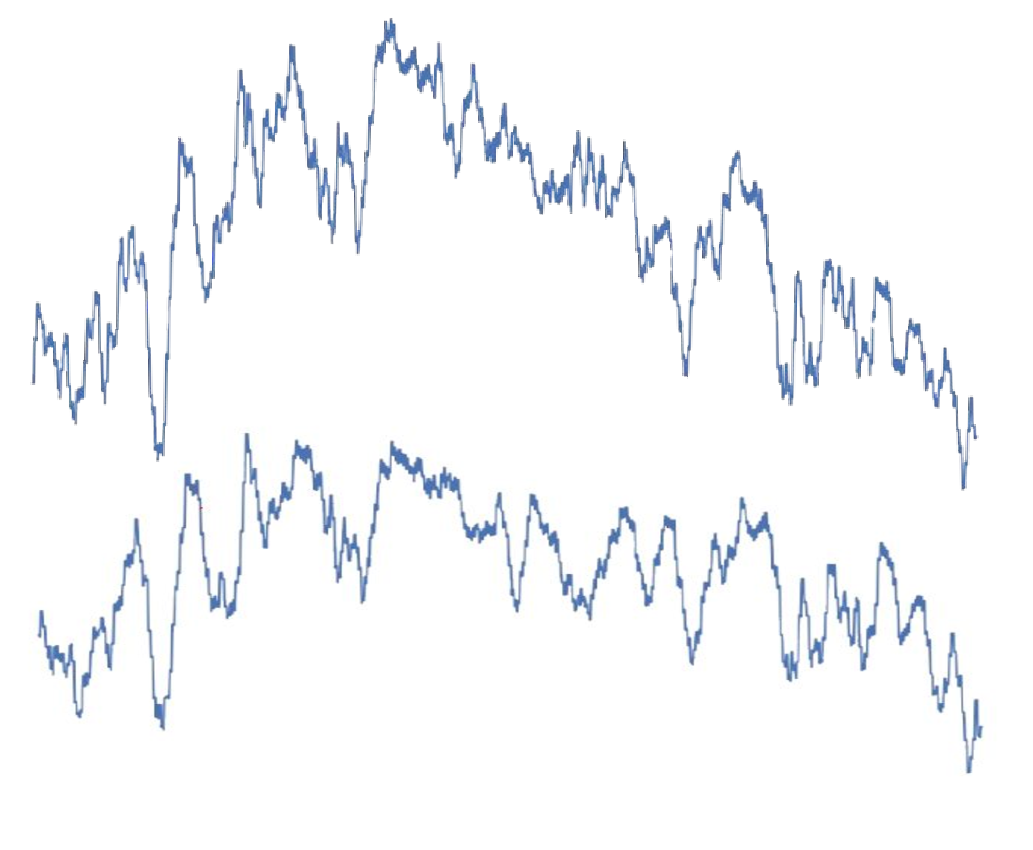
\includegraphics[width=\linewidth]{Images/misc/solar_distrib_shift.pdf}\\
        (b) Spatial shift.
    \end{minipage}
    \hfill
    \begin{minipage}[t]{0.31\textwidth}
        \centering
        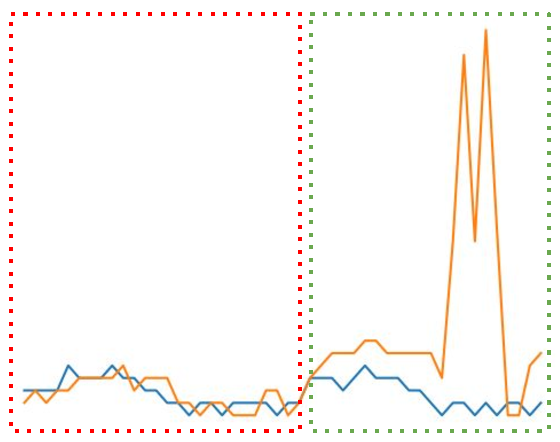
\includegraphics[width=\linewidth]{Images/misc/cond_shift_ecl.pdf}\\
        (c) Conditional shift.
    \end{minipage}
    \caption{Illustration of the three distribution shifts: (a) temporal
    shift between training and test periods (rolling average of a
    \textsc{Traffic} sensor), (b) spatial shift between users (two
    \textsc{Solar} sensors), and (c) conditional shift (different horizons
    for similar look-back windows from one \textsc{Electricity} user).}
    \label{fig:shifts}
\end{figure}


%\clearpage

In deep learning, a common approach is to apply \textit{standard normalization} to all data points, using a single global mean $\mu$ and standard deviation $\sigma$ computed empirically over the training data. Each data point is processed by subtracting the mean and dividing by the standard deviation. However, this global normalization fails to address the challenges of the three distribution shifts
%(i), (ii) and (iii)
described above
\citep{adaptivenorm}. Indeed, the statistics estimated on the training data may no longer be valid at inference. A more sophisticated and widely adopted normalization strategy is \textit{instance normalization}, which normalizes input windows using their individual statistics. This ensures that whatever the scale and offset of the input, all windows seen by the model will be similarly distributed. This method was introduced to the forecasting community as \textit{Reversible Instance Normalization} (RevIN) \citep{revin}.

The RevIN method has been adopted in numerous recent forecasting studies \citep{patchtst,fits,tirex,HUANG2025114036,revin}. Its authors argue that RevIN mitigates the distribution shift problem in time series. In this work, we investigate this claim more closely.
Our contributions are summarized as follows:
\begin{itemize}
    \item We review normalization techniques for neural forecasters and identify the key challenges they face in time series applications.
    \item We conduct extensive ablation studies on RevIN using standard forecasting benchmarks and show which components are truly necessary.
    \item We discuss the effects of instance normalization on input and output data distributions and highlight the limitations of RevIN.
    % \item We claim the \textit{conditional shift between look-back and horizon windows} remains an open challenge, and draw perspectives on how to address it.
\end{itemize}

\newpage
\section{Setting}

In this section, we formally introduce the task of time series forecasting and the distributional challenges it faces.

\paragraph{Time Series Forecasting} The task of time series forecasting consists in finding an optimal parameterized model $f_\theta$ of the form:
\begin{equation}
\label{eq:definition}
f_\theta:\;
\begin{array}{@{}c@{~}c@{~}l@{}}
  \mathbb{R}^{L} & \longrightarrow & \mathbb{R}^{H}, \\
x & \longmapsto & \hat{y} \approx y,
\end{array}
\qquad
\begin{aligned}
L &:\ \text{look-back window size},\\
H &:\ \text{horizon size}.
\end{aligned}
\end{equation}
where $\theta$ denotes the parameters of the model (e.g. a neural network), fitted on a training dataset $\mathcal{D}$ of $N$ pairs of windows $(x, y)$, with $x$ a past look-back window and $y$ a horizon to forecast. Naturally, the goal is to have predictions $\hat{y}=f_{\theta}(x)$ as close as possible to the ground-truth horizons $y$. We say a model \textit{generalizes} well when this is the case for unseen windows.

Equation \ref{eq:definition} corresponds to the \textit{univariate regression} setting, considered in this paper. A more general formulation could include multivariate inputs and outputs, exogenous covariates, and probabilistic predictions; nevertheless, we expect the main conclusions to carry over to these settings.
%, we do not consider it here.

\paragraph{Distribution shifts}
Formally, let $\mathcal{P}^{\mathcal{I},\mathcal{T}}_{X,Y}$ denote the distribution of windows corresponding to series (users / sensors) $\mathcal{I}$, during the time period $\mathcal{T}$. Temporal and spatial shifts occur when the marginal distribution $\mathcal{P}^{\mathcal{I},\mathcal{T}}_{X}$ varies across different time periods in $\mathcal{T}$ and different users in $\mathcal{I}$, respectively. They are particular examples of \textit{covariate shift} \citep{kairouz2021advances} as they describe changes in input distributions. Conditional shift occurs when the conditional distribution
$\mathcal{P}^{\mathcal{I},\mathcal{T}}_{Y|X}$ varies across $\mathcal{I}$ or $\mathcal{T}$.  It corresponds to a \textit{concept drift} \citep{moreno2012unifying}, and describes a change in the expected output for a given input. When learning a forecasting model, we typically sample examples from a subset of users $\mathcal{I}_{train}$ and a fixed time period $\mathcal{T}_{train}$. We refer to generalization as the capacity of the model to perform well for new users $\mathcal{I}_{test}$ and at a future time period $\mathcal{T}_{test}$. In case of temporal, spatial, and conditional shifts, input normalization aims to improve generalization.
